\documentclass[11pt]{article}
\usepackage{graphicx,listings}
\graphicspath{ {./images/} }
\title{\textbf{IoT 2023 Challenge 3}}
\author{
  Pasquale Castiglione\\
	\texttt{10657816}
  \and
  Lorenzo Campana\\
  \texttt{10605775}
}
\date{}
\begin{document}
\maketitle

\section*{Introduction}
The goal of this challenge was to implement a routing algorithm in order to be able to send a packet from Mote1 to Mote2.
\begin{figure}[h]
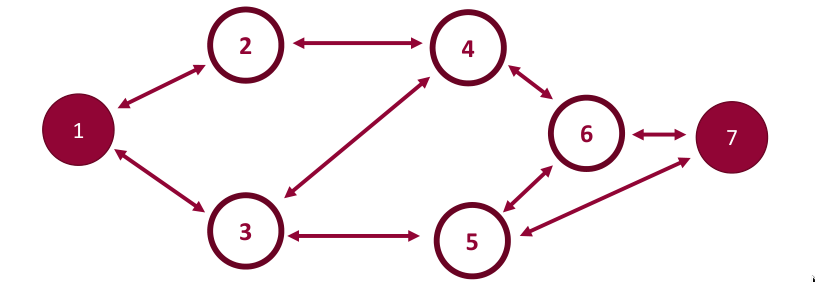
\includegraphics[width=\textwidth]{topology.png}
\caption{Network Topology}
\end{figure}
\section*{Code}
\subsection*{RadioRoute.h}
In the header file, the data structures for the messages and for the routing table were defined.
\begin{lstlisting}[language=C,basicstyle=\footnotesize]
typedef nx_struct radio_route_msg {
	nx_uint16_t type;
	nx_uint16_t sender;
	nx_uint16_t destination; // node_requested
	nx_uint16_t value; // cost
} radio_route_msg_t;
\end{lstlisting}

\begin{lstlisting}[language=C,basicstyle=\footnotesize]
typedef struct route_entry_t {
	uint16_t next_hop;
  	uint16_t cost;
} route_entry_t;
\end{lstlisting}

\subsection*{RadioRouteC.nc}
\subsubsection*{Variables} 
\texttt{waiting\_packet} and \texttt{waiting\_address} were defined in order to store the content and the destination address of the message to be sent when the routing table is empty.
\subsubsection*{Functions}
\begin{itemize}
	\item{\texttt{initializeRoutingTable}}
	\item{\texttt{addRoutingEntry}}
	\item{\texttt{dbgPacketInfo}}
\end{itemize}

\subsubsection*{Send Event}
The sending of a message is implemented in the 	\texttt{actual\_send} function.
Before the sending of a message, the variable \texttt{locked} is evaluated in order to check if the radio module is in use or not.
If the radio is free, the sending node checks if a route for the destination is present in its routing table.
In case of data message with null entry in the routing table, \texttt{waiting\_packet} and \texttt{waiting\_address} are set and a routing request sent in broadcast.
\subsubsection*{Receive Event}
Received messages are handled according to their type:
\begin{itemize}
	\item{\textbf{Data Message}}\\
		If the receiver is not the intended destination of a message then it checks if a route to the destination is present in its routing table. If a route is present then it forwards the message to the next hop.
	\item{\textbf{Route Request}}\\
		If the receiver node is the intended destination of a route request or if the node has a non empty entry in the routing table, then it answers back sending a \texttt{Route Reply} broadcast message.
		Otherwise it broadcast again the route request message to its neighbors.
		
	\item{\textbf{Route Reply}}\\
		When a \texttt{Route Reply} is received the nodes check their routing table and they update them if the received cost for the destination is lower than the stored one.
		Also, the nodes check weather there is a \texttt{waiting\_packet} with a \texttt{waiting\_address} equals to the updated entry destination address.
		In this case, it proceeds with the packet forwarding to the updated next hop.
\end{itemize}
\subsection*{Led Control}
\section*{Results}
\end{document}
